% 
%            ,,                                        
%          `7MM            _.o9                                
%            MM                                             
%  ,6"Yb.    MM  ,p6"bo   ,6"Yb.  M"""MMV  ,6"Yb.  `7Mb,od8 
% 8)   MM    MM 6M'  OO  8)   MM  '  AMV  8)   MM    MM' "' 
%  ,pm9MM    MM 8M        ,pm9MM    AMV    ,pm9MM    MM     
% 8M   MM    MM YM.    , 8M   MM   AMV  , 8M   MM    MM     
% `Moo9^Yo..JMML.YMbmd'  `Moo9^Yo.AMMmmmM `Moo9^Yo..JMML.   
% 
% 
% Free and Open-Source template for academic works
% https://github.com/dpmj/alca



\clearpage
\cleardoublepage

\chapter{Sviluppi futuri}

Un ampio spettro di sviluppi futuri è stato individuato nella cornice di questo lavoro di tesi. La pipeline di \glsname{ml} per i modelli GeneFusion può essere ulteriormente migliorata impiegando tecniche altamente sofisticate per garantire: la distribuzione portabile del sistema come applicativo \glsname{kubernetes} via \glsname{helm}; la data governance via \glsname{fybrik}; e la resilienza e affidabilità della piattaforma con metodologie di \glsname{mlre}.

\section{Distribuzione di GeneFusion come applicazione Helm}

L'orchestrazione di applicazioni complesse in ambienti Kubernetes è una sfida intrinseca, richiedendo strumenti efficaci per semplificare il processo di distribuzione e gestione. In questo contesto, Helm si erge come una soluzione chiave per facilitare la distribuzione di applicazioni su Kubernetes. Helm, un package manager per Kubernetes, offre un sistema di gestione dei pacchetti chiamati "charts" che consentono di definire, installare e aggiornare applicazioni complesse in modo coerente. L'efficacia di Helm nel coordinare e orchestrare le risorse Kubernetes si traduce in una maggiore efficienza operativa, consentendo agli sviluppatori di concentrarsi maggiormente sulla logica dell'applicazione e meno sulla complessità della distribuzione \cite{helm_official}.

Un esempio chiaro dell'utilità di Helm può essere espresso attraverso un breve snippet di codice che definisce e installa un chart. Ad esempio, il seguente snippet crea un chart di base per un'applicazione web:

\begin{code}
\captionof{listing}{Esempio di chart Helm}
\label{code:apx:a:yaml}
\begin{minted}{yaml}
# File: myapp-chart/values.yaml
    replicaCount: 2
    image:
      repository: myapp-repo
      tag: latest
    
# File: myapp-chart/templates/deployment.yaml
    apiVersion: apps/v1
    kind: Deployment
    metadata:
      name: {{ include "myapp-chart.fullname" . }}
      labels:
        app: {{ include "myapp-chart.name" . }}
    spec:
      replicas: {{ .Values.replicaCount }}
      template:
        metadata:
          labels:
            app: {{ include "myapp-chart.name" . }}
        spec:
          containers:
            - name: myapp
              image: "{{ .Values.image.repository }}:{{ .Values.image.tag }}"
              ports:
                - containerPort: 80
    
\end{minted}
\end{code}

Il passaggio da una pipeline Kubeflow a un chart Helm è un'evoluzione naturale per ottimizzare la gestione delle risorse e semplificare il processo di deployment. Trasformare una pipeline Kubeflow in un chart Helm consente di unificare e semplificare la gestione delle risorse distribuite, consentendo una transizione fluida tra fasi di sviluppo, test e produzione. Questa sinergia tra Kubeflow e Helm non solo semplifica la gestione dell'intero ciclo di vita delle applicazioni basate su machine learning ma contribuisce anche a una maggiore scalabilità e flessibilità nell'implementazione di soluzioni intelligenti \cite{kubeflow_helm_integration}.

\begin{figure}[h]
    \centering
    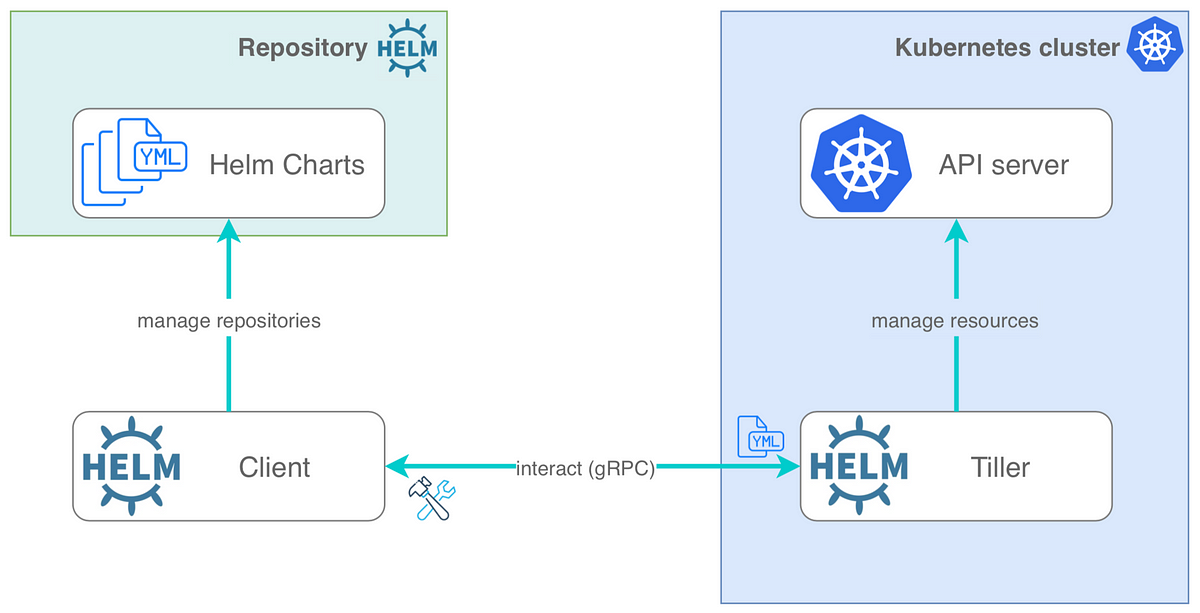
\includegraphics[width=\linewidth]{figures/ch6/helm.png}
    \caption[Impiego di Helm per distribuire applicazioni Kubernetes]{Impiego di Helm per distribuire applicazioni Kubernetes}
    \label{fig:cha6:helm}
\end{figure}

Helm rappresenta una risorsa cruciale per semplificare la distribuzione di applicazioni complesse su Kubernetes, migliorando l'efficienza operativa e permettendo agli sviluppatori di concentrarsi sulla logica dell'applicazione. La sua sinergia con Kubeflow offre un approccio olistico per ottimizzare la gestione delle risorse in scenari complessi, evidenziando l'importanza della collaborazione tra strumenti specializzati per garantire una deployment pipeline fluida e affidabile \cite{helm_kubeflow_collaboration}.

\section{Kubeflow Data Governance con Fybrik}

La gestione delle informazioni personalmente identificabili (\glsname{pii}) riveste un ruolo di fondamentale importanza nei contesti di produzione, dove la sicurezza e la conformità normativa sono prioritarie. Le PII, costituite da dati personali come nomi, indirizzi e numeri di identificazione, sono soggette a normative rigorose, poiché il loro utilizzo improprio può avere conseguenze significative sulla privacy degli individui. L'implementazione efficace di misure di protezione delle PII non solo si traduce in un adempimento alle normative, ma rappresenta anche una pietra miliare nella costruzione di fiducia con gli utenti e nel mantenimento dell'integrità delle operazioni aziendali \cite{pii_importance}.

\begin{figure}[h]
    \centering
    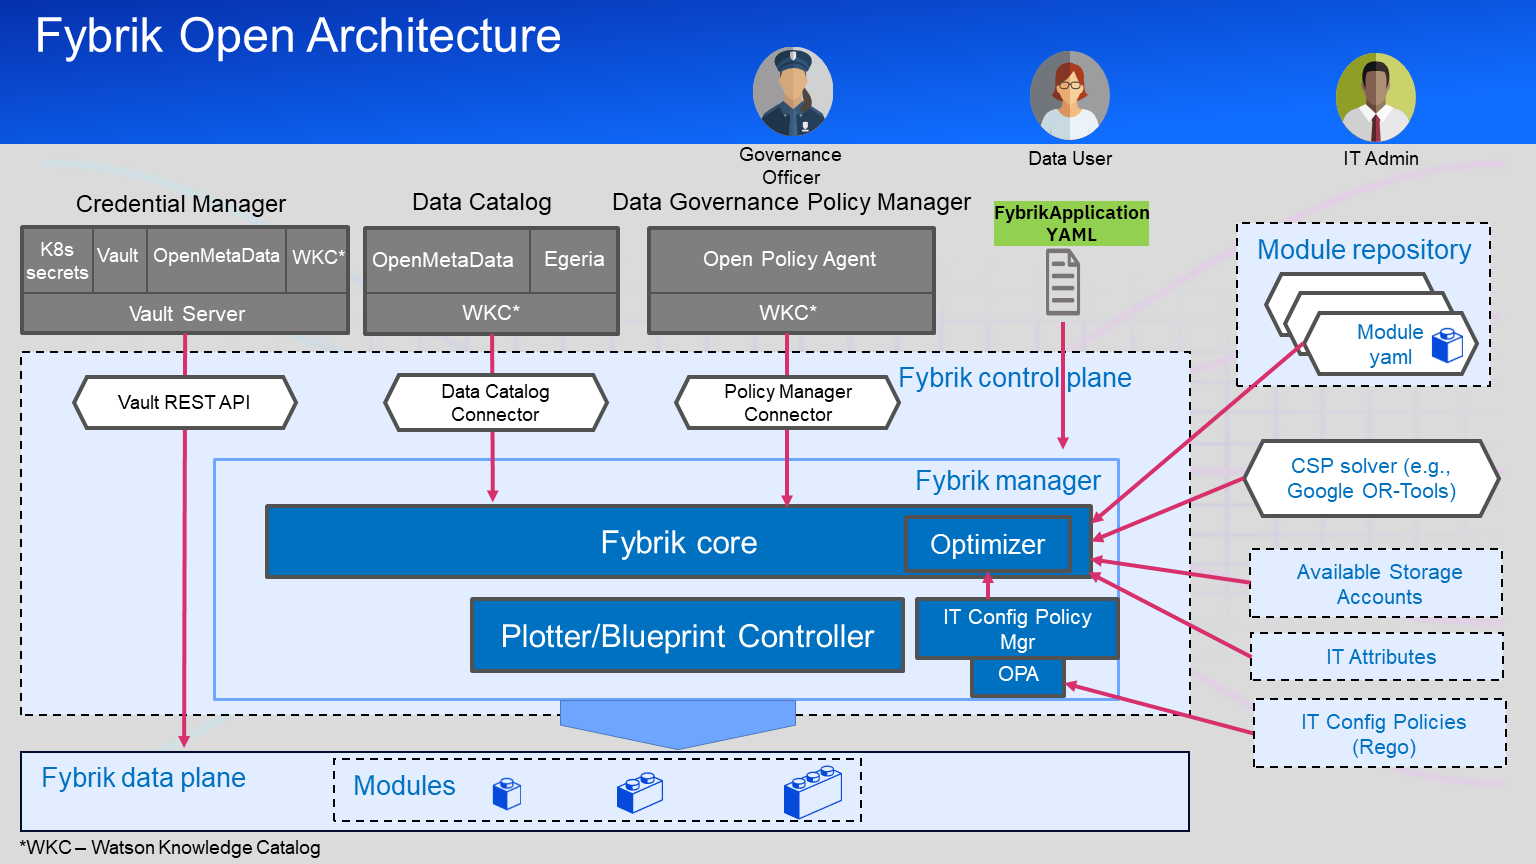
\includegraphics[width=\linewidth]{figures/ch6/fybrik.png}
    \caption[Architettura di Fybrik]{Architettura di Fybrik}
    \label{fig:cha6:fybrik}
\end{figure}

\glsname{fybrik}, nato come risposta alle crescenti sfide della gestione dei dati sensibili, si configura come un framework innovativo per la gestione sicura e decentralizzata delle informazioni. Questo strumento si propone di risolvere problemi connessi alla privacy e alla governance dei dati, offrendo un'architettura che permette l'accesso e l'elaborazione dei dati solo agli utenti autorizzati, garantendo al contempo la conformità alle normative sulla privacy come il GDPR. Fybrik sfrutta approcci di zero-knowledge proof e consent management per proteggere la riservatezza delle PII in ambienti distribuiti, consentendo alle organizzazioni di sfruttare i vantaggi del cloud senza compromettere la sicurezza dei dati \cite{fybrik_origin}.

Nel contesto di una pipeline Kubeflow, l'integrazione di Fybrik apre scenari promettenti per la gestione sicura e distribuita delle PII. Kubeflow, come piattaforma di orchestrare per il machine learning, beneficia dell'approccio di Fybrik nella gestione dei dati sensibili, garantendo che solo gli utenti autorizzati possano accedere, analizzare e utilizzare tali informazioni. L'adozione congiunta di Fybrik e Kubeflow non solo migliora la sicurezza, ma promuove anche l'efficienza nella gestione dei dati sensibili, consentendo alle organizzazioni di sfruttare appieno le potenzialità del machine learning in contesti operativi sensibili \cite{kubeflow_fybrik_integration}.

In conclusione, la salvaguardia delle PII assume un ruolo centrale nelle considerazioni operative, richiedendo soluzioni innovative come Fybrik per affrontare le sfide emergenti. L'integrazione di Fybrik in una pipeline Kubeflow rappresenta un passo significativo verso un ecosistema di machine learning che coniuga sicurezza, conformità normativa ed efficienza operativa, delineando un futuro in cui la gestione responsabile dei dati personali è al centro delle pratiche aziendali \cite{pii_security_ml}.

\section{Tecniche di Machine Learning Reliability Engineering (MLRE)}

L'avvento del \glsname{mlre} (Machine Learning Reliability Engineering) è stato motivato dall'esigenza di affrontare le sfide emergenti legate alla scalabilità, alla manutenzione e alla gestione affidabile dei modelli di machine learning in ambienti operativi complessi. La crescente diffusione dell'applicazione di algoritmi di apprendimento automatico in scenari reali ha evidenziato la necessità di garantire la robustezza e l'affidabilità dei modelli, spingendo gli esperti di machine learning a sviluppare approcci ingegneristici specifici per mitigare i rischi associati. L'MLRE ha, dunque, radici profonde nella necessità di affrontare le sfide operative, garantendo che i modelli di machine learning siano in grado di gestire scenari del mondo reale in modo coerente e affidabile \cite{MLRE_origin}.

Un esempio della possibile implementazione di pratiche MLRE è rappresentato dall'integrazione all'interno di una pipeline Kubeflow. Kubeflow, come piattaforma open-source, offre un ambiente orchestrato per la gestione end-to-end delle attività di machine learning, facilitando lo sviluppo, la distribuzione e la scalabilità dei modelli. L'implementazione di tecniche di MLRE in una pipeline Kubeflow potrebbe offrire vantaggi sostanziali in termini di monitoraggio continuo, gestione degli errori e ottimizzazione delle prestazioni. Inoltre, la natura distribuita di Kubeflow si presta bene alla parallelizzazione delle attività di MLRE, consentendo un miglioramento significativo nella gestione delle risorse e nell'adattamento dinamico alle variazioni nel contesto operativo \cite{Kubeflow_integration}.

\begin{figure}[h]
    \centering
    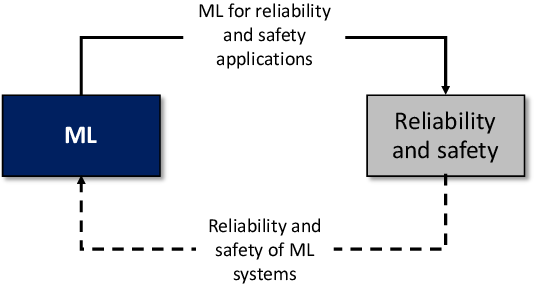
\includegraphics[width=250px]{figures/ch6/mlre.png}
    \caption[Correlazione fra Machine Learning e Reliability]{Correlazione fra Machine Learning e Reliability}
    \label{fig:cha6:mlre}
\end{figure}

La branca MLRE è emersa come risposta alle sfide sempre più complesse e critiche che caratterizzano l'integrazione dei modelli di machine learning nell'ambiente operativo. La necessità di affrontare questioni quali la gestione delle derive di dati, la degradazione delle prestazioni nel tempo e la rilevazione tempestiva di anomalie ha spinto la comunità scientifica a sviluppare un approccio ingegneristico dedicato. Attraverso l'applicazione di principi di ingegneria del software e del sistema, l'MLRE mira a garantire la coerenza e la fiducia nei modelli di machine learning, permettendo alle organizzazioni di sfruttare appieno i benefici di tali tecnologie in ambienti operativi reali.

Tuttavia, va sottolineato che l'implementazione di pratiche MLRE all'interno di Kubeflow non sarebbe priva di sfide. La complessità della gestione delle risorse distribuite, la necessità di definire metriche affidabili per la valutazione della fiducia nei modelli e la progettazione di politiche di fallback robuste sono solo alcune delle questioni che richiedono un'attenzione particolare. La collaborazione tra la comunità MLRE e gli sviluppatori di Kubeflow diventa, pertanto, cruciale per garantire un'integrazione armoniosa e un continuo miglioramento delle capacità operative.

L'MLRE si configura dunque come un pilastro fondamentale per la creazione e la gestione di modelli di machine learning affidabili in scenari reali, mentre l'integrazione con Kubeflow apre nuove prospettive per una distribuzione efficiente e sicura. La convergenza di queste discipline indica una prospettiva promettente per l'evoluzione delle pratiche di sviluppo e implementazione di soluzioni di machine learning, sottolineando l'importanza di un approccio ingegneristico orientato alla fiducia e alla robustezza nei confronti dei sistemi intelligenti \cite{MLRE_Kubeflow_integration}.